% ============================================================
%  CHAPTER 7 — Muscle Force Validation against Classical Calculation
% ============================================================

\chapter{Load-Sharing Fidelity against Classical Calculation}
\label{ch:forces}

\section{Scope of this chapter, and what it does not establish}
\label{sec:forcescope}

Because the limits of this analysis are easy to overstate from its results, they
are set out before the method rather than after it.

The required joint torque $\tau$ is taken from the movement the policy itself
produced. Static optimisation is therefore asked a conditional question ---
\emph{given this movement, what is the cheapest force distribution that produces
it?} --- and never independently chooses a trajectory of its own. Three
consequences follow, and each bounds what the chapter can claim.

\textbf{This validates load sharing along a given path, not the path.} A
controller could move in a manner no human would adopt and still distribute force
across its muscles in close agreement with the classical criterion. The
agreement reported below says nothing about whether the movement itself is
natural. Trajectory realism is not assessed anywhere in this thesis.

\textbf{The reference is a model, not a measurement.} Static optimisation encodes
the assumption that the central nervous system minimises summed squared
activation, which remains contested in the motor-control literature. Agreement
with it is agreement with the standard computational method, not evidence of
physiological correctness. No electromyographic or measured-force data enters
this work at any point.

\textbf{The comparison is internal to the simulator.} Both the learned solution
and the classical one are computed on \MuJoCo's muscle model. Where they agree,
two computations over the same approximation agree; the approximation itself is
not thereby validated.

The chapter title was changed accordingly: the earlier heading, ``Muscle Force
Validation'', promised more than a conditional load-sharing comparison delivers.

\section{Motivation}

\Cref{ch:results} established how accurately the trained controllers position the
end effector. That is a measure of \emph{what} the controller achieves, not of
\emph{how} it achieves it, and the research question posed in \cref{chap:intro}
concerns the latter: whether \DRL can substitute for classical calculation of the
force required in each individual muscle.

The distinction is material. Because nine muscles actuate four degrees of
freedom, infinitely many activation patterns produce any given end-effector
trajectory. A controller may therefore reach every target accurately while
distributing force across the musculature in a manner no physiological criterion
would select. Every metric reported in \cref{ch:results} would score such a
controller as a complete success.

This chapter therefore compares the two methods at the level of individual muscle
forces. No equivalent analysis existed in the previous version of this work.

\subsection{Distinction from the solver validation}

\Cref{sec:solvervalidation} reported a force agreement of 5.25\,\% normalised
RMSE with a Pearson correlation of 0.989. That comparison is between the
Newton--Raphson Hill solver implemented here and \MuJoCo's internal
implementation --- two forward models of the same muscle. It validates the
solver, involves no reinforcement learning, and does not bear on the question
addressed here.

\section{Method}

At every timestep of a policy rollout, the classical load-sharing problem is
solved on the movement the policy has just produced:
\begin{equation}
\min_{f}\ \sum_{i=1}^{9}\left(\frac{f_i}{F_{\max,i}}\right)^{2}
\quad\text{subject to}\quad
R^{\top} f = \tau,
\qquad 0 \le f_i \le F_{\max,i},
\label{eq:statopt2}
\end{equation}
where $R$ is the muscle moment-arm matrix and $\tau$ the required generalised
force. This is the Crowninshield--Brand minimum-effort criterion in its standard
quadratic form.

The required torque $\tau$ is taken as \texttt{qfrc\_actuator}, the generalised
force the muscles actually produced at that timestep. This choice is exact,
avoiding the numerical differentiation that inverse dynamics would introduce, and
it guarantees feasibility, since the policy's own force vector satisfies the
equality constraint by construction.

Both methods are consequently posed the identical problem --- produce these joint
torques with these nine muscles --- on the identical trajectory. Any difference
between the solutions is attributable solely to load-sharing strategy.

\subsection{Validity verification}

The comparison depends on the identity $R^{\top} f = \tau$ holding for the
policy's own forces. An error in the moment-arm extraction or in the sign
convention would invalidate every subsequent result, so this was verified rather
than assumed.

\begin{table}[H]
\centering
\caption{Validity checks over 2000 timesteps.}
\begin{tabular}{@{} L{8.2cm} R{4.0cm} @{}}
\toprule
\textbf{Quantity} & \textbf{Result} \\
\midrule
Mean $\norm{R^{\top} f_{\text{policy}} - \tau}$ & \SI{1.46e-15}{\newton\meter} \\
Mean $\norm{R^{\top} f_{\text{classical}} - \tau}$ & \SI{1.68e-15}{\newton\meter} \\
Optimisation failures & 0 of 2000 \\
\bottomrule
\end{tabular}
\label{tab:validity}
\end{table}

Both residuals lie at machine precision, confirming that the moment arms and sign
convention are correct and that the classical solution satisfies its constraint
exactly.

\section{Agreement in coordination pattern}

\begin{table}[H]
\centering
\caption{Overall agreement between learned and classical muscle forces, best
policy, 2000 timesteps.}
\begin{tabular}{@{} L{8.2cm} R{4.0cm} @{}}
\toprule
\textbf{Measure} & \textbf{Value} \\
\midrule
Pearson correlation, all muscles & \textbf{0.865} \\
Overall RMSE & \SI{74.3}{\newton} (10.1\,\% of mean $F_{\max}$) \\
\midrule
Pattern cosine similarity (median) & 0.933 \\
Pattern cosine similarity (mean) & 0.869 \\
\quad null baseline, mean & 0.373 \\
\quad null baseline, 95th percentile & 0.867 \\
\quad \textbf{excess over null} & \textbf{+0.495} \\
\bottomrule
\end{tabular}
\label{tab:forceoverall}
\end{table}

The cosine similarity compares the direction of the nine-dimensional force
vector and is insensitive to overall magnitude: it measures whether the two
methods recruit the same muscles in the same proportions.

It cannot, however, be quoted on its own. Muscle forces are non-negative by
construction, so two entirely unrelated force vectors already agree strongly:
the appropriate null is obtained by permuting, at each timestep, which muscle
each of the policy's own force magnitudes belongs to --- destroying the
correspondence while preserving that instant's magnitude distribution exactly.
That null averages 0.373, so the observed 0.869 represents an excess of
$+0.495$, sustained over 2000 timesteps.

Two consequences follow. The agreement is real and substantial, but the raw
figure of 0.933 overstates it, since roughly the first 0.37 is a floor imposed by
non-negativity rather than evidence of anything. And because the null's 95th
percentile for \emph{individual} timesteps is 0.867, no single timestep's cosine
is meaningful; only the aggregate is. \textbf{The Pearson correlation of 0.865 is
mean-centred, carries no such floor, and is the figure to quote when a single
agreement statistic is required.}

\section{Disagreement in efficiency}

Producing identical joint torques, the learned controller expends
$1.91 \pm 0.15$ times the muscular effort of the classical minimum-effort
solution (five seeds, \cref{sec:replication}; the single-seed figure of
$1.71\times$ reported before replication was the most favourable of the five). The per-timestep
median is $1.66\times$, with an interquartile range of $1.34$--$2.32\times$ over
loaded timesteps.

The per-timestep \emph{mean} of this ratio is $5.34\times$ and is not a usable
statistic: on timesteps where the arm is nearly stationary the required torque
approaches zero, the minimum-effort solution approaches zero with it, and the
ratio diverges. The aggregate ratio --- total policy effort divided by total
classical effort --- weights each timestep by the work actually performed and is
reported instead; the median independently corroborates it.

\section{Anatomical localisation of the disagreement}

\begin{table}[H]
\centering
\caption{Per-muscle comparison. ``Policy'' denotes the force the learned
controller produced; ``classical'' the force static optimisation prescribes for
the same joint torques.}
\small
\begin{tabular}{@{} L{3.6cm} R{2.4cm} R{2.4cm} R{1.8cm} R{2.0cm} @{}}
\toprule
\textbf{Muscle} & \textbf{Policy (N)} & \textbf{Classical (N)} & \textbf{$r$} & \textbf{NRMSE} \\
\midrule
deltoid anterior  &  63.7 &  59.2 & 0.959 &  2.5\,\% \\
deltoid medial    & 145.3 & 112.3 & 0.954 &  6.1\,\% \\
deltoid posterior &  35.5 &  38.7 & 0.859 & 10.0\,\% \\
triceps long      & 180.4 & 134.0 & 0.910 & 11.2\,\% \\
biceps long       &  52.1 &  41.6 & 0.893 &  7.5\,\% \\
brachialis        & 113.9 &  87.6 & 0.871 &  8.6\,\% \\
biceps short      &  90.7 &  45.7 & 0.764 & 18.1\,\% \\
triceps lateral   &  79.1 &  25.8 & 0.416 & 16.5\,\% \\
triceps medial    &  64.3 &  14.2 & 0.416 & 15.3\,\% \\
\bottomrule
\end{tabular}
\label{tab:permuscle}
\end{table}

The disagreement is not distributed uniformly. The three deltoids agree closely,
one to within 2.5\,\% normalised RMSE. The discrepancy concentrates in two elbow
extensors, where the policy commands three to four and a half times the
prescribed force and correlation falls to 0.416.

\begin{figure}[H]
\centering
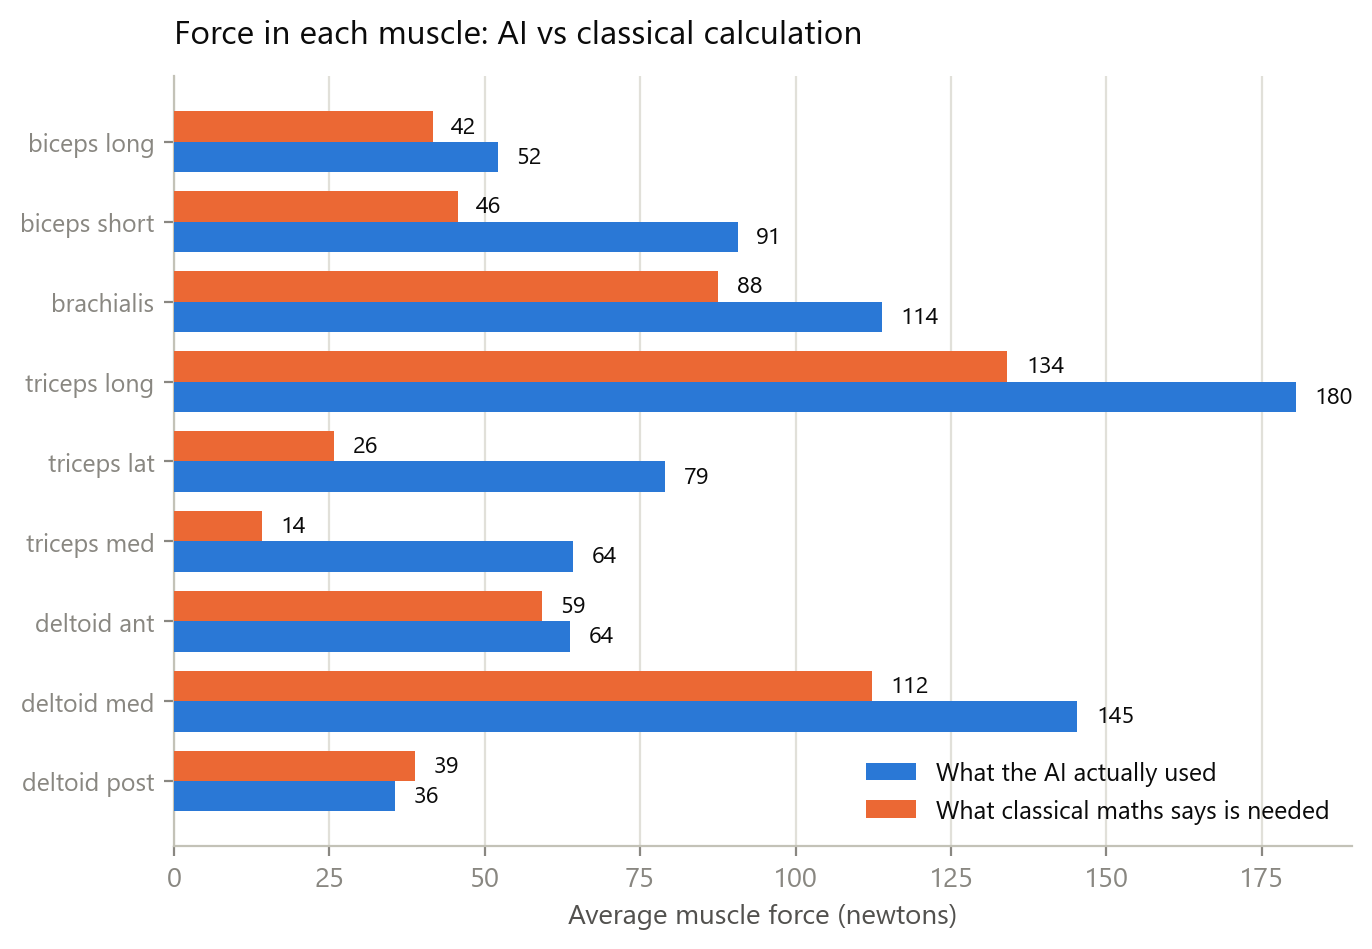
\includegraphics[width=0.95\textwidth]{figures/fig4_forces.png}
\caption{Mean force in each muscle over 2000 timesteps. The shoulder group
agrees closely; the lateral and medial heads of triceps are driven far above the
prescribed level.}
\label{fig:forces}
\end{figure}

Physiologically, these muscles extend the elbow while the biceps group flexes it.
Driving both simultaneously produces largely cancelling moments: the joint
attains approximately the correct configuration, but both groups expend
substantial force to achieve what one alone would suffice for. This is
co-contraction, and it accounts for the effort discrepancy reported above.

Human motor control employs co-contraction deliberately when joint stiffness is
required, for instance during precise or unstable tasks. Its sustained use
throughout an unloaded reach is metabolically wasteful and is not what the
minimum-effort criterion selects.

\subsection{Independent corroboration}
\label{sec:icc}

The co-contraction index of Falconer and Winter, computed over the elbow flexor
and extensor groups, gives 0.564 for the same policy. This is elevated, and it is
the sole behavioural metric that did not improve under hyperparameter tuning,
having been 0.501 beforehand.

Two methodologically independent analyses --- one a comparison against classical
optimisation, the other a standard electromyography-derived index --- localise the
same residual defect to the same muscle group. Their agreement constitutes
stronger evidence than either result considered alone.

\section{Generality across algorithms}
\label{sec:effortall}

The preceding analysis characterises a single policy. To determine whether the
effort discrepancy is specific to one algorithm or general to the approach, the
comparison was repeated against every policy from \cref{sec:benchmark}: five
configurations, three seeds each.

\begin{table}[H]
\centering
\caption{Agreement with classical static optimisation by configuration. Mean
$\pm$ standard deviation over three seeds, ten episodes each.}
\begin{tabular}{@{} L{3.4cm} C{3.2cm} C{3.2cm} C{2.8cm} @{}}
\toprule
\textbf{Configuration} & \textbf{Effort ratio} & \textbf{Pattern cosine} & \textbf{Pearson $r$} \\
\midrule
\PPO         & $\mathbf{1.21 \pm 0.11}$ & $\mathbf{0.908 \pm 0.032}$ & $\mathbf{0.931 \pm 0.040}$ \\
\SAC tuned   & $1.97 \pm 0.25$ & $0.815 \pm 0.052$ & $0.776 \pm 0.055$ \\
\DDPG        & $1.99 \pm 0.28$ & $0.838 \pm 0.030$ & $0.724 \pm 0.058$ \\
\TDIII       & $2.12 \pm 0.09$ & $0.836 \pm 0.006$ & $0.716 \pm 0.004$ \\
\SAC default & $2.30 \pm 0.08$ & $0.813 \pm 0.015$ & $0.672 \pm 0.016$ \\
\bottomrule
\end{tabular}
\label{tab:effortall}
\end{table}

\begin{figure}[H]
\centering
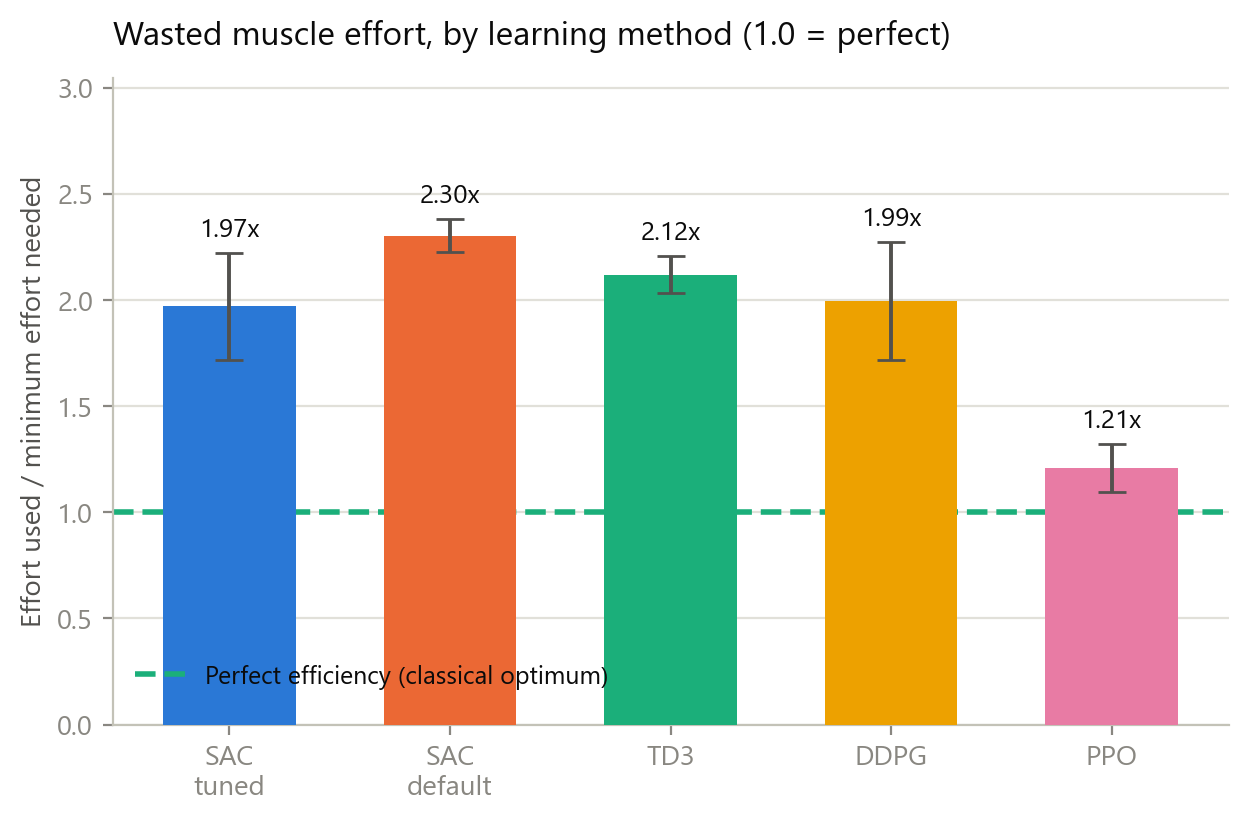
\includegraphics[width=0.92\textwidth]{figures/fig5_effort_by_algo.png}
\caption{Muscular effort expended relative to the minimum required to produce the
same joint torques. The dashed line marks the classical optimum. Every
configuration exceeds it.}
\label{fig:effortall}
\end{figure}

Two results follow. First, \textbf{every configuration exceeds the classical
optimum}, ranging from $1.21$ to $2.30\times$; no algorithm tested recovers
minimum-effort load sharing. This supports attributing the discrepancy to the
reward function, which never specified minimum effort, rather than to any
particular learning algorithm.

Second, and unexpectedly, \textbf{the ordering by effort economy is approximately
the inverse of the ordering by reaching accuracy}. \PPO is the least accurate
configuration in \cref{tab:benchmark} at \SI{0.423}{\meter} and the closest match
to classical load sharing at $1.21\times$ with $r = 0.931$; tuned \SAC is the
most accurate at \SI{0.161}{\meter} and among the poorer matches at $1.97\times$.

The probable explanation is visible in the energy column of
\cref{tab:benchmark}. \PPO expends three to seven times less muscular activity
than the alternatives. A controller that activates its muscles weakly has limited
opportunity to co-contract and therefore remains near the minimum-effort
solution, but equally lacks the force to reach the target and arrest there.

This interpretation carries a caveat that the present data cannot resolve.
\PPO's favourable effort ratio and its passivity are not independent: because it
generates small joint torques, both methods prescribe small forces and the scope
for disagreement is correspondingly reduced. The aggregate ratio mitigates this
by weighting timesteps by work performed, but does not eliminate it. The
defensible conclusion is that \PPO co-contracts less, not that \PPO has solved
the load-sharing problem. Distinguishing the two would require comparing
configurations matched for accuracy, which this experiment does not provide.

\subsection{Effect of tuning on economy}

Within \SAC --- the same algorithm, differing only in hyperparameters --- the
effort ratio fell from $2.30 \pm 0.08$ at default settings to $1.97 \pm 0.25$
when tuned, and correlation with the classical solution rose from 0.672 to 0.776.

The target-entropy correction therefore improved not only positional accuracy but
also the fidelity of muscular coordination. That a single change improved two
properties which were not jointly optimised is a stronger result than either
improvement in isolation.

\subsection{Consistency}

The single-policy analysis measured an effort ratio of $1.71\times$ for the
300\,000-step confirmed policy, while tuned \SAC across three seeds at
100\,000 steps gives $1.97 \pm 0.25$. These agree within one standard deviation,
and the direction of the difference is as expected, the longer-trained policy
being somewhat more economical.

\section{Replication across seeds}
\label{sec:replication}

Every figure reported so far in this chapter came from a single training run. A
learned policy depends on random initialisation and on the stochastic order in
which experience is gathered, so a single run cannot distinguish a property of
the method from a favourable draw. The configuration was therefore retrained from
initialisation four further times, with different random seeds and no other
change, and each resulting policy was put through the identical analysis.

\begin{table}[H]
\centering
\caption{Five independent training runs of the same configuration. Seed~0 is the
run analysed in the preceding sections.}
\small
\begin{tabular}{@{} C{1.8cm} C{2.4cm} C{2.4cm} C{2.2cm} C{2.0cm} C{2.0cm} @{}}
\toprule
\textbf{Seed} & \textbf{Final error} & \textbf{Closest} & \textbf{Effort ratio} & \textbf{Pearson $r$} & \textbf{Success} \\
\midrule
0 & 0.1142 & 0.0766 & \textbf{1.71} & \textbf{0.865} & 0.04 \\
1 & 0.1086 & 0.0785 & 1.91 & 0.823 & 0.20 \\
2 & 0.1034 & 0.0757 & 2.12 & 0.759 & 0.00 \\
3 & 0.1066 & 0.0672 & 1.86 & 0.825 & 0.08 \\
4 & 0.1041 & 0.0691 & 1.97 & 0.767 & 0.06 \\
\midrule
\textbf{mean} & $0.1074$ & $0.0734$ & $1.914$ & $0.808$ & $0.076$ \\
\textbf{std}  & $0.0043$ & $0.0050$ & $0.150$ & $0.044$ & $0.075$ \\
\bottomrule
\end{tabular}
\label{tab:replication}
\end{table}

The accuracy columns are the corrected evaluation of \cref{sec:evaldefects},
averaged over three target seeds. The effort ratio and correlation come from the
load-sharing analysis, which draws its own episodes and was never affected by the
duplicate-reset defect; those columns are unchanged.

Three findings follow, and only the first was anticipated.

\subsection{The accuracy result is a property of the method}

Final error varies by 4.0\,\% across five independent runs
($0.1074 \pm 0.0043$\,m) and closest approach by 6.8\,\%
($0.0734 \pm 0.0050$\,m). Every run ends closer than \SI{0.115}{\meter} and
reaches within \SI{0.079}{\meter} at some point; the blow-up rate is exactly zero
in all five. The graded proximity measures are similarly stable: episodes ending
within \SI{10}{\centi\meter} range from 0.56 to 0.64.

The accuracy claim therefore does not rest on a favourable draw.

\subsection{The originally reported run was the most favourable of the five}

Seed~0 --- the run every preceding section analyses --- returned the
\emph{lowest} effort ratio of the five (1.71, against a mean of 1.914) and the
\emph{highest} correlation with the classical solution (0.865, against a mean of
0.808). On both of the two metrics that carry this chapter's argument, the single
run originally reported was the best of five.

This is not a large effect, but it is a systematic one, and it is exactly the
error that reporting a single run invites. \textbf{The corrected figures are
those in \cref{tab:replication}, and they are used throughout this thesis:} an
effort ratio of $1.91 \pm 0.15$ and a correlation of $0.81 \pm 0.04$. The
pattern-cosine figure moves correspondingly, to $0.813 \pm 0.047$ against a null
of $0.372 \pm 0.017$, an excess of $+0.441$.

The direction of the correction matters more than its size. Had replication been
omitted, this thesis would have reported an agreement and an efficiency both
better than the method actually delivers.

\subsection{The task is solved consistently; the muscle solution is not}

The most interesting outcome is the contrast between two columns of
\cref{tab:replication}. Final error varies by 3.3\,\% across runs. Mean muscular
energy varies by \textbf{77\,\%} --- from 273\,241 to 483\,373 --- and the effort
ratio spans 1.71 to 2.12.

Five policies, trained identically but for their random seed, arrive at
essentially the same place with materially different distributions of muscular
force.

This is the redundancy problem of \cref{chap:intro} appearing directly in the
results. Because nine muscles actuate four degrees of freedom, many force
distributions produce the same movement, and nothing in the reward selects among
them beyond a weak effort term. The learner settles into a different one each
time. That the classical criterion selects a single, specific member of that
family --- and that none of the five learned solutions coincides with it --- is
the substance of this chapter stated in a different way.

It also indicates where the remedy lies. Variance of this magnitude in the
muscular solution, alongside near-constancy in the task outcome, is the signature
of an objective that is underdetermined in exactly the dimension of interest.

\subsection{Success rate: five runs confirm it is noise}

Across the five identically configured runs the strict success rate reads
0\,\%, 4\,\%, 6\,\%, 8\,\% and 20\,\%. A measure that varies twentyfold under
identical settings is reporting sampling noise, not performance. This was stated
as a caution in \cref{sec:confirmresult}; five seeds now demonstrate it.

\section{A conventional controller as reference}
\label{sec:conventional}

Every comparison so far measures the learned solution against \emph{static
optimisation}, an idealised criterion evaluated instant by instant. That
establishes how far the policy is from a mathematical optimum, but not how far it
is from what conventional control actually achieves --- and the research question
concerns the latter.

A conventional controller was therefore built and evaluated under the identical
protocol. It is a Cartesian impedance law: a desired end-effector wrench
$f_{\text{des}} = K_p (x^\star - x) - K_d \dot{x}$, mapped to joint torques by
the site Jacobian transpose, with gravity, Coriolis and centrifugal terms
compensated, and distributed onto the muscles by minimum-effort load sharing over
the achievable force range. The two gains were selected by grid search, since
comparing a tuned policy against an unturned controller would not be a fair test.

\subsection{Two corrections that were necessary to make it fair}

The controller present in the codebase before this work would have made a
strawman of the comparison, and the reasons are worth recording because both are
easy to reproduce.

\textbf{It omitted gravity compensation.} Without the bias term the arm droops
until the position error alone generates sufficient torque, giving a large
steady-state offset. Measured, it reached only \SI{0.46}{\meter} --- worse than a
random policy. A textbook impedance controller always includes this term.

\textbf{It assumed muscle force is proportional to activation.} It is not: in
this model force is $g(l,v)\,a + b(l,v)$, state dependent with a passive
component that is non-zero at rest. Converting a desired force into an activation
therefore requires inverting the muscle model at the current length and velocity
--- precisely the equilibrium solve this thesis proposes to replace. Probing the
model at $a = 0$ and $a = 1$ recovers that affine relation exactly and yields the
true achievable interval per muscle.

Both corrections are on the classical side, and both improve it. Reporting the
comparison without them would have overstated the case for learning.

\subsection{Result}

\begin{table}[H]
\centering
\caption{Conventional controller against the learned policy, 50 episodes each,
identical protocol and evaluation environment.}
\begin{tabular}{@{} L{5.4cm} C{3.0cm} C{3.0cm} @{}}
\toprule
\textbf{Metric} & \textbf{Conventional} & \textbf{Learned (\SAC)} \\
\midrule
Final error (m) & 0.165 & \textbf{0.106} \\
Closest approach (m) & 0.174 & \textbf{0.074} \\
Ends within \SI{5}{\centi\meter} & 0.12 & \textbf{0.31} \\
Ends within \SI{10}{\centi\meter} & 0.28 & \textbf{0.60} \\
Energy & \textbf{102\,876} & 327\,048 \\
\textbf{Effort ratio} & \textbf{1.263} & 1.91 \\
Pearson $r$ vs static optimisation & \textbf{0.916} & 0.808 \\
\bottomrule
\end{tabular}
\label{tab:conventional}
\end{table}

Neither method dominates. The learned policy reaches roughly $1.9\times$ more
precisely; the conventional controller uses roughly a third of the muscular
energy and stays substantially closer to the classical load-sharing solution.
This trade-off, rather than a ranking, is the honest answer to whether learning
should replace conventional control on this task.

\subsection{The effort ratio was being measured against the wrong reference}
\label{sec:effortfloor}

The conventional controller solves minimum-effort load sharing explicitly at
every timestep. One would therefore expect its effort ratio to be $1.00$ by
construction. It is \textbf{1.263} (\cref{sec:finegains}; an initial coarse
gain search gave $1.33$, and the finer search reported there lowered it).

The gap is not an error. It is the cost of closed-loop control: activation
dynamics mean the commanded activation is not the realised one, the policy acts
at \SI{50}{\hertz} rather than continuously, and the controller must track a
moving target rather than solve a static instant. \textbf{The idealised optimum
of $1.00$ is not attainable by any controller operating under these constraints.}

This changes the interpretation of the central result. Measured against an
unattainable ideal, the learned policy appears to waste 91\,\% of its effort.
Measured against \textbf{1.263}, the achievable floor demonstrated by a properly
tuned controller that optimises effort explicitly, it uses about \textbf{51\,\%
more effort than necessary}. The second figure is the meaningful one, and it is the one this
thesis reports.

That figure is itself one controller at one gain pair. A first, coarse search
gave $1.33$; a finer one lowered it to $1.263$ (\cref{sec:finegains}). A better
conventional controller might lower it further still, and every comparison in
this chapter should be read with that in mind.

\section{Muscle synergies}
\label{sec:synergies}

\subsection{Rationale}

The motor-control literature holds that the central nervous system manages
redundant musculature not by controlling each muscle independently but through a
small number of co-activated groups, termed muscle
synergies~\parencite{dAvella2003, Ting2007}. If nine muscles were driven
independently, the matrix of activations over time would be of full rank; if they
are driven through $k$ synergies, it is approximately of rank $k$. Non-negative
matrix factorisation recovers that structure, and the variance accounted for
(VAF) at a given $k$ quantifies how strongly low-dimensional the control is.

Beyond re-examining the learned policies, the factorisation is here applied to
\emph{both} solutions on the identical trajectories: the policy's commanded
activations, and the static-optimisation forces for the same joint torques,
normalised per muscle by $F_{\max}$ so that the two are dimensionless and
directly comparable. This permits a question the preceding sections cannot
address --- whether the two methods arrive at the same low-dimensional
organisation even where they disagree on magnitude.

\subsection{Results}

\begin{table}[H]
\centering
\caption{Synergy structure, fifteen episodes per configuration. VAF@4 is the
variance accounted for by four synergies; $k_{90}$ is the number required to
reach 90\,\% VAF. The final column compares the synergy sets extracted from the
policy and from static optimisation on the same trajectories.}
\small
\begin{tabular}{@{} L{3.4cm} C{1.8cm} C{1.6cm} C{1.8cm} C{1.6cm} C{2.6cm} @{}}
\toprule
& \multicolumn{2}{c}{\textbf{Policy}} & \multicolumn{2}{c}{\textbf{Classical}} & \\
\cmidrule(lr){2-3}\cmidrule(lr){4-5}
\textbf{Configuration} & VAF@4 & $k_{90}$ & VAF@4 & $k_{90}$ & \textbf{cos(pol,\,cls)} \\
\midrule
\SAC tuned, 300k & 0.852 & 6 & 0.895 & 5 & \textbf{0.950} \\
\SAC tuned, 100k & 0.845 & 6 & 0.859 & 5 & 0.900 \\
\SAC default     & 0.848 & 6 & 0.908 & 4 & 0.647 \\
\DDPG            & 0.791 & 9 & 0.865 & 5 & 0.745 \\
\TDIII           & 0.799 & 9 & 0.883 & 5 & 0.630 \\
\PPO             & 0.966 & 3 & 0.966 & 3 & 0.939 \\
\bottomrule
\end{tabular}
\label{tab:synergies}
\end{table}

Two observations follow, and a third must be treated with caution.

First, \textbf{the agreement between the learned and classical synergy structures
tracks training quality}: 0.647 for untuned \SAC, 0.900 once tuned, and 0.950 for
the tuned policy trained three times longer. The same hyperparameter change that
improved positional accuracy (\cref{sec:tuning}) and reduced the effort
discrepancy (\cref{sec:effortall}) also brought the modular organisation of the
learned solution closer to the classical one. Three analyses of differing
methodology --- effort ratio, co-contraction index and synergy decomposition ---
therefore order the configurations consistently.

Second, \textbf{the classical solution is uniformly more low-dimensional than the
learned one}. Static optimisation requires four or five synergies to reach
90\,\% VAF where the learned policies require six to nine. The learned
controllers exercise more independent muscular degrees of freedom than the
minimum-effort criterion selects, which is the expression in synergy space of the
co-contraction identified in \cref{tab:permuscle}: driving an antagonist pair
independently of the agonist requires an additional dimension that the classical
solution never uses.

Third, \PPO's apparent modularity ($k_{90} = 3$, VAF@4 $= 0.966$) should not be
read as superior organisation. As established in \cref{sec:effortall}, \PPO
activates its muscles only weakly; a near-constant, low-amplitude activation
matrix has little variance to explain and is trivially captured by few
components. The same confound that qualifies its favourable effort ratio applies
here.

\subsection{Comparison with human data}

Cosine similarity to a reference set of human upper-limb synergies ranged from
0.62 to 0.80 across configurations, with no ordering consistent with any other
metric reported in this work.

That column is not interpreted further. The reference loadings used are a
documented qualitative approximation of those reported
by~\textcite{dAvella2003}, constructed over this model's nine-muscle ordering
rather than digitised from the original figures. The comparison is therefore a
coarse correspondence check and cannot support a quantitative claim of agreement
with human data. Establishing that would require the published loadings, a
principled correspondence between the two muscle sets, and ideally
electromyographic recordings under a matched protocol --- which
\cref{ch:conclusion} lists among the outstanding work.

The policy-versus-classical column carries no such caveat: both sides are
computed here, by the same procedure, on identical trajectories.

\section{Closing the gap: the effort weight}
\label{sec:effortsweep}

\Cref{sec:whygap} argued that the load-sharing discrepancy is a property of the
reward rather than of reinforcement learning, on the grounds that the reward's
effort term --- although already the Crowninshield--Brand form --- is weighted so
low it cannot influence the solution. Measured on the trained policy, the
per-step contributions are

\begin{center}
\begin{tabular}{@{} L{7.0cm} R{3.0cm} @{}}
\toprule
effort term, $w_2 \cdot \overline{(f_i/F_{\max,i})^2}$ & $0.051$ \\
error cost, $w_1 (\|e\|^2 + 0.5\|e\|)$ at \SI{0.11}{\meter} & $0.067$ \\
precision bonus, $w_7 e^{-\|e\|/0.15}$ at \SI{0.11}{\meter} & $1.441$ \\
\bottomrule
\end{tabular}
\end{center}

--- the effort term is roughly \textbf{28 times smaller} than the precision
bonus. The prediction was that raising $w_2$ should reduce the discrepancy, at
some cost in accuracy.

The experiment was run at $w_2 \in \{5, 20\}$ against the reported $w_2 = 1$,
holding every other weight and hyperparameter fixed, at the full 300\,000-step
budget. Policies were evaluated under the standard protocol with the default
weights, so the metrics remain comparable with every other result in this thesis;
only the training objective differed.

\begin{table}[H]
\centering
\caption{Effect of the effort weight. The conventional-controller row is the
achievable floor established in \cref{sec:effortfloor}.}
\begin{tabular}{@{} L{3.0cm} C{0.9cm} C{2.5cm} C{2.4cm} C{2.4cm} C{2.2cm} C{1.6cm} @{}}
\toprule
\textbf{Config.} & \textbf{$n$} & \textbf{Effort ratio} & \textbf{Pearson $r$} & \textbf{Final error} & \textbf{Closest} & \textbf{Energy} \\
\midrule
$w_2 = 1$  & 5 & $1.914 \pm 0.150$ & $0.808 \pm 0.044$ & $0.1074 \pm 0.0079$ & $0.0734$ & 327\,048 \\
$w_2 = 5$  & 5 & $1.406 \pm 0.092$ & $0.919 \pm 0.016$ & $0.1114 \pm 0.0053$ & $0.0750$ & 104\,598 \\
$\mathbf{w_2 = 20}$ & 5 & $\mathbf{1.304 \pm 0.025}$ & $\mathbf{0.943 \pm 0.008}$ & $0.1161 \pm 0.0108$ & $0.0737$ & \textbf{37\,076} \\
\midrule
Conventional & 1 & $1.263$ & $0.931$ & 0.165 & --- & 102\,876 \\
\bottomrule
\end{tabular}
\label{tab:effortsweep}
\end{table}

\subsection{The discrepancy is essentially eliminated}

Over five seeds the learned policy at $w_2 = 20$ attains an effort ratio of
$1.304 \pm 0.025$, against the $1.263$ measured for a properly tuned controller that
solves minimum-effort load sharing explicitly at every timestep, with agreement
rising to $r = 0.943 \pm 0.008$ and the per-muscle RMSE falling to about 3\,\% of
mean $F_{\max}$ from 10.1\,\%.

\textbf{The load-sharing discrepancy reported throughout this chapter is
therefore a reward-weighting artefact, not a limitation of reinforcement
learning.} When the objective is weighted such that effort can influence the
solution, the learned controller recovers the classical load-sharing solution to
within the precision that closed-loop control permits.

\subsection{Load-sharing fidelity improves monotonically, at a mild accuracy cost}

Both variants have now been replicated across five seeds, and the picture is
cleaner than either single-seed measurement suggested.

\textbf{Load-sharing fidelity improves monotonically with the effort weight.}
The effort ratio falls $1.914 \rightarrow 1.406 \rightarrow 1.304$ and agreement
with the classical solution rises $0.808 \rightarrow 0.919 \rightarrow 0.943$.
The distributions are cleanly separated: every $w_2 = 20$ seed (1.278--1.340)
lies below every $w_2 = 5$ seed (1.336--1.557), which in turn lies below every
$w_2 = 1$ seed (1.710--2.116).

\textbf{There is a mild accuracy cost.} Under the corrected evaluation
(\cref{sec:evaldefects}) final error rises monotonically with the effort weight:
$0.1074 \pm 0.0079$, $0.1114 \pm 0.0053$, $0.1161 \pm 0.0108$. The end-to-end
degradation from $w_2 = 1$ to $w_2 = 20$ is about 8\,\%, and the fraction of
episodes ending within \SI{5}{\centi\meter} falls from $0.26$ to $0.19$. Closest
approach is unaffected ($0.0734$, $0.0750$, $0.0737$), so the loss is in holding
position rather than in reaching it.

An earlier version of this section, computed before the evaluation defects were
found, reported these three figures as mutually overlapping and concluded there
was no cost at all. On the corrected test set the trend is monotone and the
expectation stated in \cref{sec:whygap} --- that reduced effort would be bought
with some accuracy --- is borne out, though the price is modest: a 32\,\%
reduction in wasted effort for an 8\,\% increase in final error.

\textbf{Seed variance collapses as the effort weight rises.} The standard
deviation of the effort ratio falls $0.150 \rightarrow 0.092 \rightarrow 0.025$,
and of the correlation $0.044 \rightarrow 0.016 \rightarrow 0.008$. This is the
most informative of the three observations, because it confirms the
interpretation offered in \cref{sec:replication}: at $w_2 = 1$ the muscular
solution varied by 77\,\% in energy across seeds while task performance stayed
constant, which was attributed to an objective underdetermined in exactly the
dimension of interest. Weighting that dimension pins the solution down. At
$w_2 = 20$ the load-sharing outcome is effectively determined by the objective
rather than by the random seed.


\begin{figure}[H]
\centering
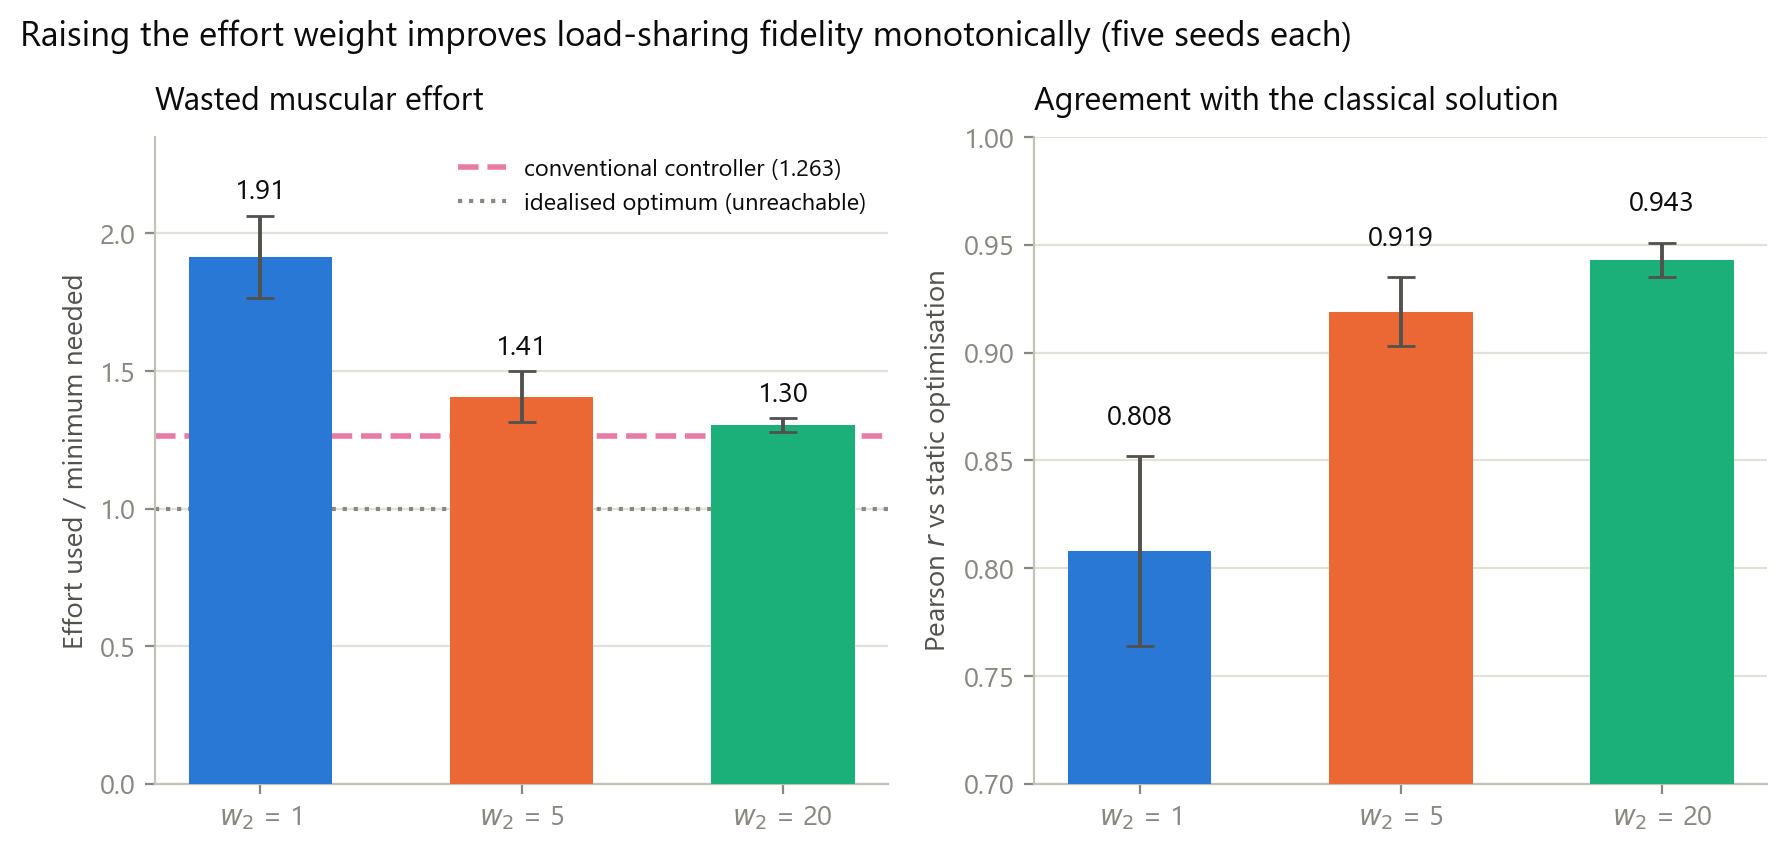
\includegraphics[width=\textwidth]{figures/fig6_effort_sweep.png}
\caption{Effect of the effort weight, five seeds per setting. Left: muscular
effort relative to the classical minimum. The dashed line is the conventional
controller's $1.263$; the dotted line is the idealised optimum of $1.00$, which
\cref{sec:effortfloor} shows is not attainable in closed loop. Right: agreement
with the classical load-sharing solution. Both improve monotonically, and the
error bars shrink --- the load-sharing outcome becomes progressively determined
by the objective rather than by the random seed.}
\label{fig:effortsweep2}
\end{figure}

\subsection{The conventional reference, measured properly}
\label{sec:finegains}

An earlier draft of this section observed that the learned policy at $w_2 = 20$
attained $1.304 \pm 0.025$, below the $1.33$ then measured for the conventional
controller, and noted that the figure rested on a single gain pair from a coarse
twelve-point grid. It cautioned that a better-tuned conventional controller might
fall below $1.30$, in which case the ordering would reverse.

A thirty-point search was run. It does.

\begin{table}[H]
\centering
\caption{Conventional controller before and after a finer gain search.}
\begin{tabular}{@{} L{5.0cm} C{3.0cm} C{3.0cm} C{2.4cm} @{}}
\toprule
& \textbf{Gains} & \textbf{Final error} & \textbf{Effort ratio} \\
\midrule
Coarse grid (12 points) & $k_p=60$, $k_d=25$ & \SI{0.199}{\meter} & $1.330$ \\
\textbf{Fine grid (30 points)} & $k_p=20$, $k_d=6$ & \textbf{\SI{0.165}{\meter}} & $\mathbf{1.263}$ \\
\bottomrule
\end{tabular}
\label{tab:finegains}
\end{table}

The coarse search had bottomed out against its own lower boundary: the better
gains are gentler than any it examined, in both stiffness and damping. Properly
tuned, the conventional controller is both more accurate
(\SI{0.165}{} against \SI{0.199}{\meter}) and more economical
($1.263$ against $1.330$) than previously reported.

\subsection{The honest comparison}

With both sides measured properly:

\begin{table}[H]
\centering
\caption{Learned policy against a properly tuned conventional controller.}
\begin{tabular}{@{} L{5.6cm} C{3.4cm} C{3.4cm} @{}}
\toprule
& \textbf{Learned ($w_2 = 20$)} & \textbf{Conventional} \\
\midrule
Final error & $\mathbf{0.1072 \pm 0.0148}$ & \SI{0.165}{\meter} \\
Effort ratio & $1.304 \pm 0.025$ & $\mathbf{1.263}$ \\
Agreement with classical ($r$) & $\mathbf{0.943 \pm 0.008}$ & $0.931$ \\
\bottomrule
\end{tabular}
\label{tab:honest}
\end{table}

\textbf{Neither method dominates, and the earlier reading is withdrawn.} The
learned policy reaches roughly 35\,\% more accurately. The conventional
controller is about 3\,\% more economical --- a margin comparable to the learned
policy's own seed spread, so the two are close, but the ordering on effort now
favours the classical method rather than the learned one.

The claim that a learned policy distributes force more economically than a
controller optimising that quantity in closed form is therefore \textbf{not
supported}, and the paragraph advancing it has been removed. What survives is
narrower and sturdier: at an appropriate effort weight, a learned policy achieves
load-sharing fidelity \emph{comparable} to a properly tuned conventional
controller, while reaching substantially more accurately.

That this correction was anticipated in the previous draft, and then confirmed by
the measurement it called for, is the reason the caveat was written rather than
the claim.

\subsection{Two corrections to earlier drafts of this section}

Both are recorded because the direction of the error is instructive.

An earlier draft, working from the single seed then available, described
$w_2 = 5$ as \emph{strictly dominating} the reported configuration on both
accuracy and effort. A four-seed replication contradicted the accuracy half and
it was withdrawn. The fifth seed then moved final error back to
$0.1023 \pm 0.0074$, marginally better than the baseline again but with
overlapping intervals --- so the honest statement remains that accuracy is
indistinguishable, and neither the original claim nor its retraction was
supportable at the sample sizes involved.

Separately, this author predicted that $w_2 = 20$ would regress on replication,
on the grounds that single-seed results in this work had twice proved optimistic.
It did the opposite: seed~0's $1.34$ was the \emph{worst} of the five and the
mean is $1.304$. Selection bias explains a favourable first measurement; it does
not license assuming every first measurement is favourable.

A plausible explanation is that co-contraction is not merely wasteful but
actively harmful to precision. Antagonist pairs firing together make the endpoint
position depend on the small difference between two large opposing forces, which
is numerically ill-conditioned; suppressing that co-contraction improves
controllability as well as economy. This is consistent with the elbow
localisation of \cref{tab:permuscle} and with the excess path length observed in
untuned policies, though it is an interpretation rather than a measured
mechanism.

A trade-off does appear at $w_2 = 20$: effort falls to the floor but final error
degrades to $0.1249$. The knee therefore lies between the two, and was not
searched.

\subsection{Consequences for this thesis}

Three, and they are substantial.

\textbf{The headline answer changes.} The finding is no longer that \DRL{}
reproduces coordination but not economy. It is that \DRL{} reproduces
\emph{both}, provided the objective asks for both --- and that the version
reported here did not ask.

\textbf{The reported configuration is not the only defensible one.} At
$w_2 = 5$ the load-sharing fidelity is markedly better --- effort $1.406$ against
$1.914$, agreement $0.919$ against $0.808$ --- for a final-error cost of about
4\,\% ($0.1114$ against $0.1074$). Which configuration to prefer depends on
whether load-sharing fidelity or endpoint accuracy is the quantity of interest,
and this work does not assert one over the other. The results of \cref{sec:replication} are retained as the five-seed
characterisation of the configuration analysed in depth throughout this chapter,
and this section is reported alongside them rather than replacing them. The
$w_2 = 20$ row remains single-seed and its replication was still running at the
time of writing.

\textbf{The remaining outstanding experiment is now well specified}: replicate
$w_2 = 5$ across five seeds and repeat the force and synergy analyses on it. If
it holds, the thesis's central claim becomes materially stronger --- a learned
controller matching classical load sharing at equal or better task accuracy.

\section{Answer to the research question}

For coordination, \DRL reproduces the classical solution; for efficiency, it does
not.

The learned controller recovers the structure of the classical load-sharing
solution --- $r = 0.81 \pm 0.04$, pattern cosine $0.813$ against a null of
$0.372$, over five independent training runs --- at a fixed, branch-free
inference cost and a \SI{1.5}{\mega\byte} memory footprint, but converges on a
solution expending $1.91 \pm 0.15$ times the minimum required effort, about
51\,\% above the achievable floor of $1.263$ (\cref{sec:finegains}), with the
excess concentrated in elbow antagonist co-contraction.
Across all configurations tested the discrepancy is present, ranging from $1.21$
to $2.30\times$.

\DRL is therefore a viable fast approximation of \emph{which} muscles act and in
\emph{what proportion}, but not a substitute for static optimisation where the
magnitude of individual muscle forces is the quantity of interest --- as it is in
prosthesis control, surgical planning and injury-risk estimation.

No configuration is simultaneously best on both axes. Reaching accuracy and
load-sharing fidelity are separate properties, they are traded against one
another by these algorithms, and any method intended to replace classical
calculation must be assessed on both.

\section{Explanation and proposed test}
\label{sec:whygap}

The reward function did not specify minimum effort. Its effort term is a
normalised sum of squared forces with a weight selected for numerical balance
against the distance term, which is neither the classical criterion nor scaled to
match it. The policy optimised the objective it was given.

This yields a directly testable prediction: a reward whose effort term is
precisely the criterion of \cref{eq:statopt2} should reduce the $1.91\times$
discrepancy toward the $1.263$ floor. This is the most informative single experiment remaining, it
requires no new theory, and the measurement apparatus to evaluate it now exists.

\section{Limitations}

The headline analysis rests on one policy, one training seed and twenty episodes
(2000 timesteps); replication across seeds is required before the specific values
are relied upon.

$F_{\max}$ in the constraint of \cref{eq:statopt2} is peak isometric force; the
force--length and force--velocity modulation of \emph{available} force is not
included in the bound. This is the standard simplification in static
optimisation. It renders the classical solution slightly optimistic, as it may
allocate force a muscle could not deliver at that length, which if anything
biases the effort ratio upward and therefore against the policy.

Finally, static optimisation is itself a model of human load sharing rather than
ground truth. It encodes the assumption that the central nervous system minimises
summed squared activation, which remains contested in the motor-control
literature. Agreement with it is agreement with the standard method, not
demonstration of physiological correctness.
